\documentclass[a4paper]{article}

\usepackage{cite}%多个文献引用
\usepackage{graphicx}
\usepackage{array}%调节表格行高
\usepackage{multirow,makecell}%多行表格
\usepackage{tabularx}%表格固定列宽
\usepackage{subfigure}
\usepackage{titlesec}%标题格式设置
\usepackage{amsmath}
\usepackage{amssymb}
\usepackage{tabularx}
\usepackage{makecell}
\usepackage{geometry}
\usepackage{float}
\usepackage{setspace}%行距包
\usepackage{siunitx}
\usepackage{mdwlist}
\usepackage{tabu}
\usepackage{enumerate}

\geometry{top=1.54cm,bottom=2.54cm,left=2.5cm,right=2.5cm}


\begin{document}
\begin{center}
\bf\Large
EE 105 Feedback Control Systems\par
Department of Electrical and Computer Engineering\par
Tufts University Fall 2018\par
Homework \#11\par   
\end{center}
\begin{table}[H]
\begin{center}
\begin{tabular*}{\textwidth}{@{\extracolsep{\fill}}lcr}
Name: {\it Shang Wang} &Student ID: {\it 1277417} &E-mail: {\it shang.wang@tufts.edu}\\
\hline
\end{tabular*}
\end{center}
\end{table}

% \begin{figure}[H]
% \centering
% 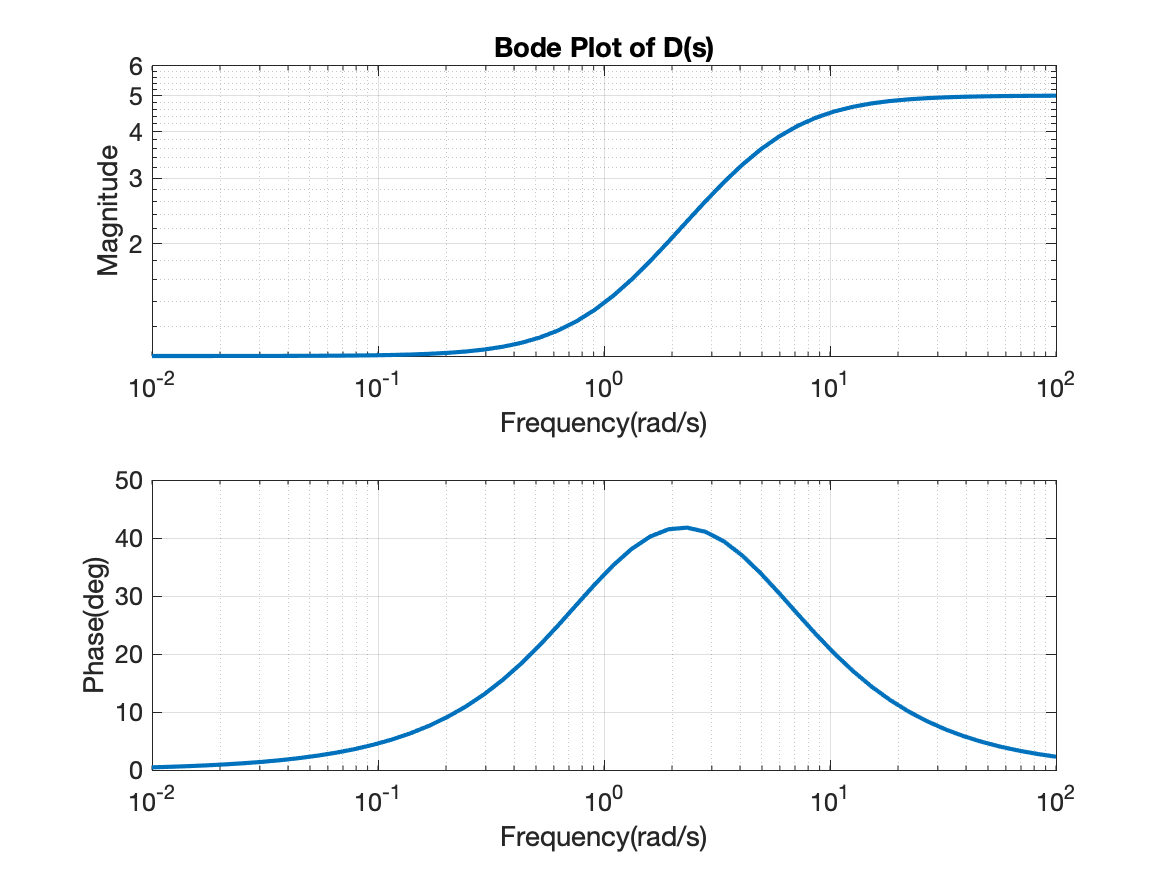
\includegraphics[width = 0.75\textwidth]{pic/0.png}
% \end{figure}

% $$
% A = 
% \left [
% \begin{matrix}
%    -1 & 0 \\
%    1 & 0
% \end{matrix}
% \right ],\ \ \
% $$

% \begin{equation*}
% f_U(u) = 
% \left\{
% \begin{aligned}
% & 0 &&,\ uL-5\\
% & \frac{u+5}{8} &&,\ -5\leq u < -3\\
% \end{aligned}
% \right.
% \end{equation*}

\section{Problem 1}
\subsection{Part A}
The state equation and the output equation:
\begin{equation*}
\begin{aligned}
& \dot{x}_1 = -5 x_1 - 4x_3 + u\\
& \dot{x}_2 = x_1\\
& \dot{x}_3 = x_2\\
& y = 100x_3
\end{aligned}
\end{equation*}
So the control matrices are:
$$
A =  \left [
\begin{matrix}
   -5 & -4 & 0 \\
   1 & 0 & 0 \\
   0 & 1 & 0 \\
\end{matrix}
\right ], \ \ \  
B = \left [
\begin{matrix}
   1 \\
   0 \\
   0 \\
\end{matrix}
\right ],\ \ \ 
C = \left [
\begin{matrix}
   1 & 0 & 0 
\end{matrix}
\right ], \ \ \ 
D = 0
$$

\subsection{Part B}
The block diagram is:
\begin{figure}[H]
\centering
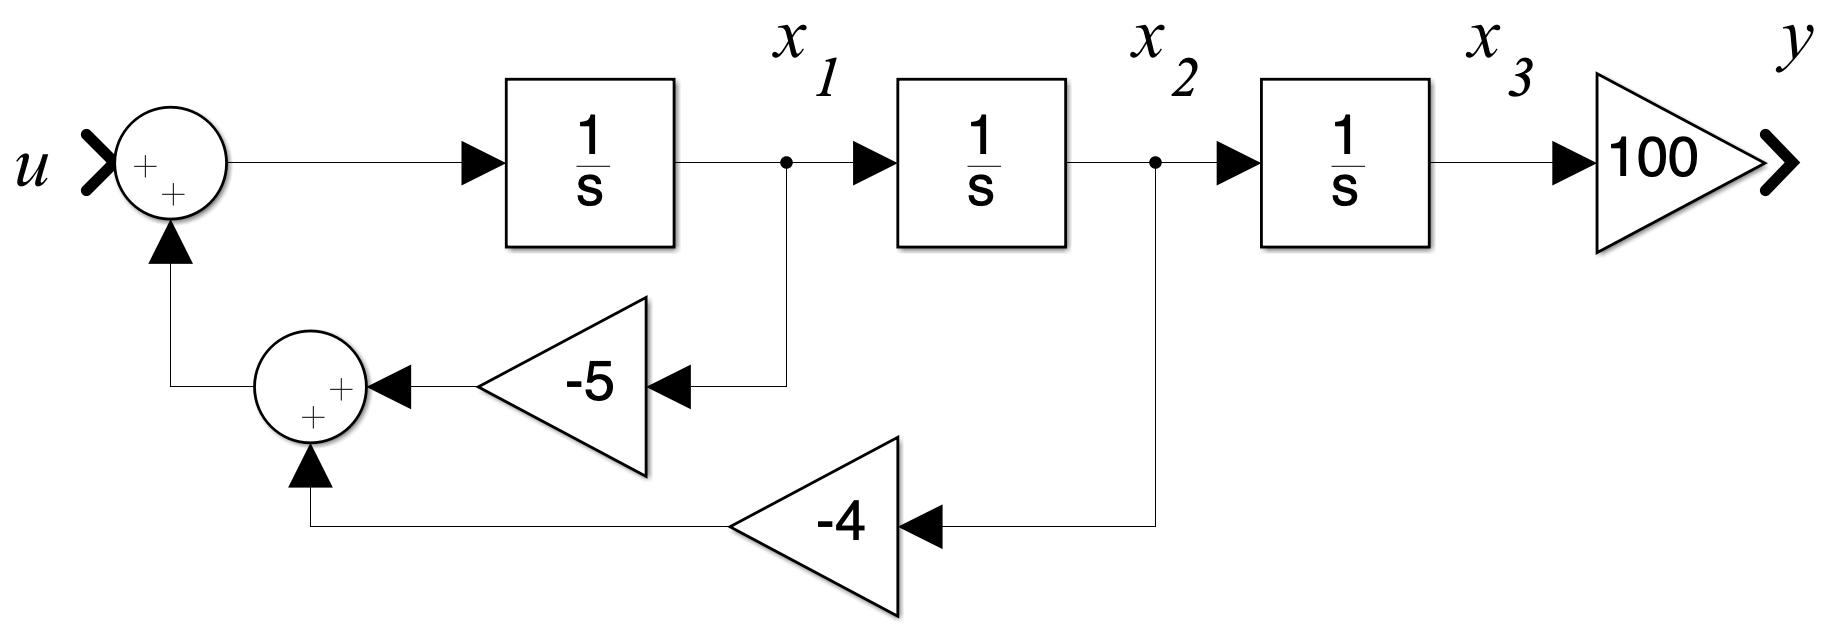
\includegraphics[width = 0.75\textwidth]{pic/1.png}
\end{figure}


\subsection{Part C}
To move the poles to $p = -1, -2, -4$, we need to calculate the characteristic polynomial:
$$
(p + 1)(p + 2)(p + 4) = p^3 + 7p^2 + 14p +8
$$
Then subtract it by characteristic polynomial of the dynamic system. then we have:
$$
K = [2,\ 10,\ 8]
$$

\subsection{Part D}
Here is the system with feadback path:
\begin{figure}[H]
\centering
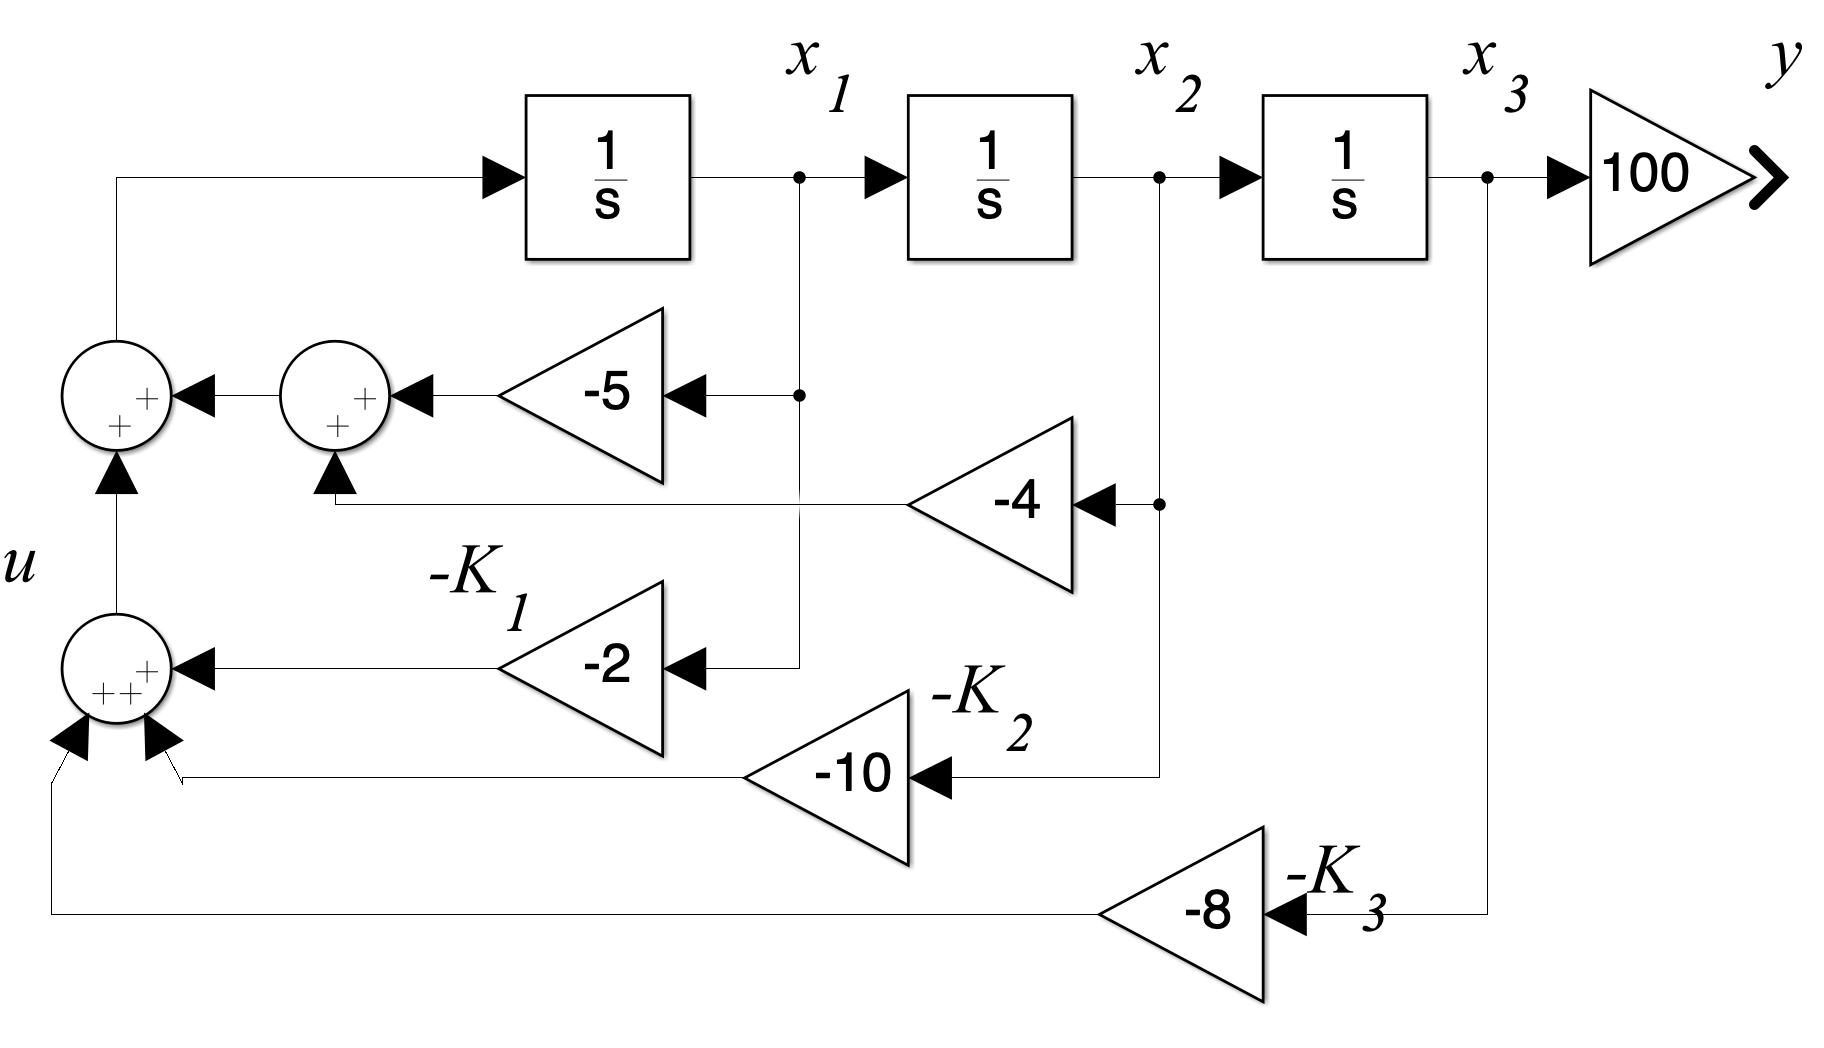
\includegraphics[width = 0.75\textwidth]{pic/2.png}
\end{figure}

\subsection{Part E}
Here is the estimator:
\begin{figure}[H]
\centering
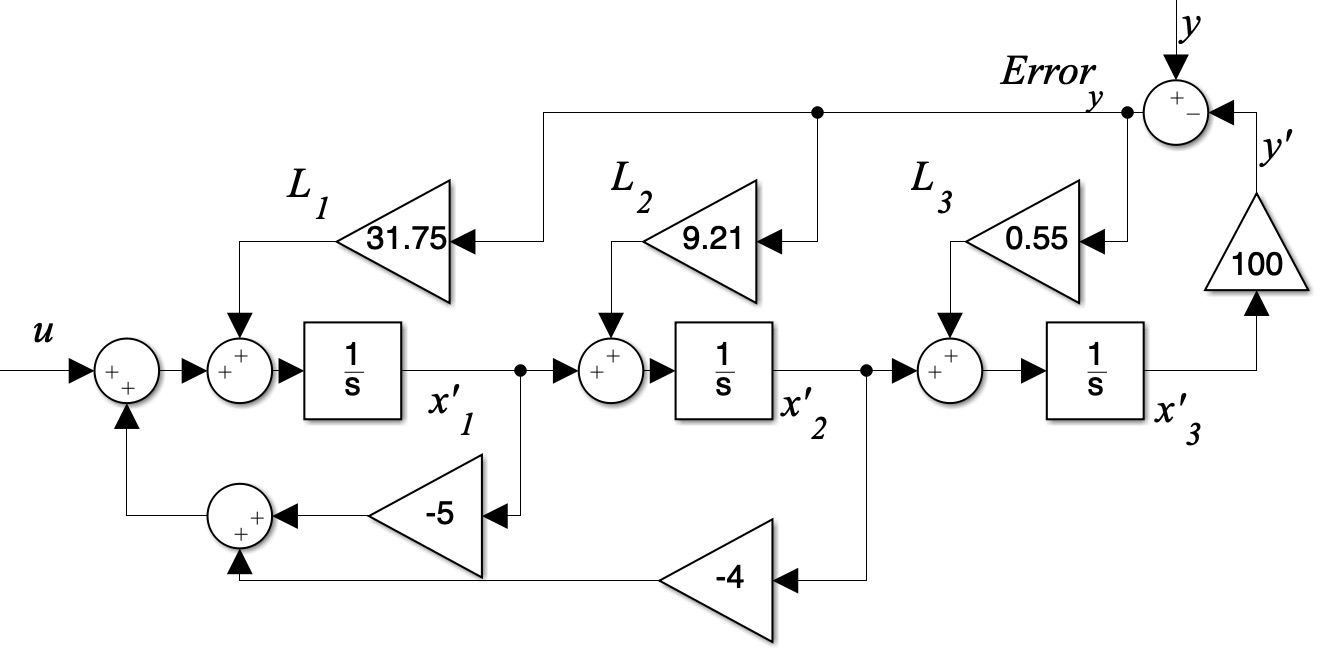
\includegraphics[width = 0.75\textwidth]{pic/3.png}
\end{figure}


\subsection{Part F}
To calculate the $L$, we need the characteristic equation of the estimator:
$$
(p+20)^3 = p^3 + 60p^2 + 1200p + 8000 = 0
$$
And the same characteristic equation could be derived in matrices form by using matrices $A,C,L$:
$$
\det[pI-(A-LC)] = 0
$$
subtitute by the numetrical value:
$$
\det\Bigg\{ 
\left [\begin{matrix}
   p & 0 & 0 \\
   0 & p & 0 \\
   0 & 0 & p \\
\end{matrix}\right ]
-\Bigg(
\left [\begin{matrix}
   -5 & -4 & 0 \\
   1 & 0 & 0 \\
   0 & 1 & 0 \\
\end{matrix}\right ]
- 
\left [\begin{matrix}
   L1\\
   L2\\
   L3\\
\end{matrix}\right ] 
\left [
\begin{matrix}
   0 & 0 & 100 
\end{matrix}
\right ]\Bigg)\Bigg\}
$$
Then we have:
$$
\det\Bigg\{
\left [\begin{matrix}
   p+5 &4 &100L_1\\
   -1 &p  &100L_2\\
   0 &-1 & p + 100L_3\\
\end{matrix}\right ] \Bigg\} = 0
$$
The characteristic equation is
$$
p^3+ (100L_3 + 5)p^2 + (4 + 100L_2 + 500L_3)p +(100L_1 + 500L_2 + 400L_3)
 = 0
$$
So we get
$$
100L_3 + 5 = 60 ,\ \ 4 + 100L_2 + 500L_3 = 1200,\ \ 100L_1 + 500L_2 + 400L_3 = 8000,\\
$$
Thus:
$$
L_1 = 31.75,\ \ L_2 = 9.21,\ \ L_3 = 0.55
$$

\subsection{Part G}
Here is the whole design:
\begin{figure}[H]
\centering
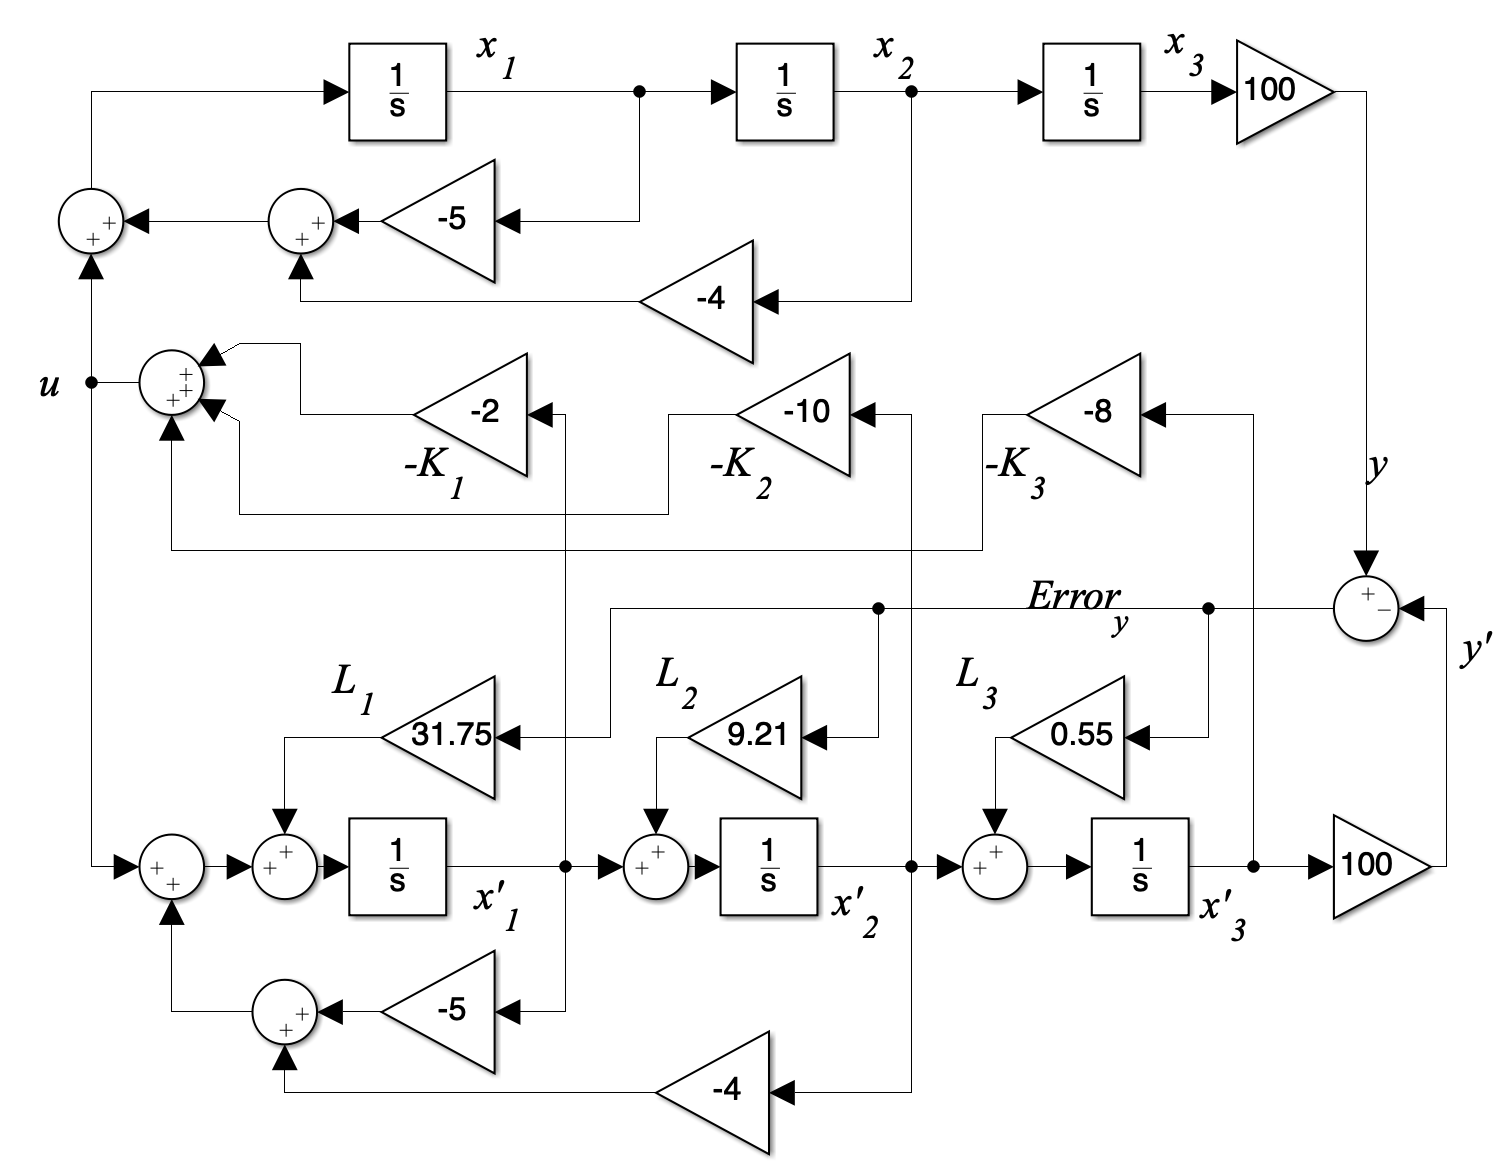
\includegraphics[width = 0.75\textwidth]{pic/4.png}
\end{figure}



\end{document}